\section{遍历二叉树及其应用}

\begin{frame}\ft{\secname}

\begin{dingyi}[遍历二叉树 - Traversing Binary Tree]
按某种次序依次访问二叉树中的所有结点,使得每个结点被访问一次且只被访问一次。
%% 所谓访问是指对结点做某种处理。如:输出信息、修改结点的值等。
\end{dingyi}

\vspace{0.1in}

\begin{zhu}
\begin{itemize}
\item \textcolor{acolor5}{关键词:} 访问和次序。\\[0.1in]
\item 访问指的是要根据实际的需要来确定具体做什么,比如对每个结点做相关计算、输出打印等。
\end{itemize}
\end{zhu}
%% 二叉树是一种非线性结构,每个结点都可能有左、右两棵子树,因此,需要寻找一种规律,使二叉树上的结点能排列在一个线性队列上,从而便于遍历。
%% 二叉树的基本组成:根结点、左子树、右子树。若能依次遍历这三部分,就是遍历了二叉树。

\end{frame}
%
%
\begin{frame}\ft{\secname}

若以L、D、R分别表示遍历左子树、遍历根结点和遍历右子树,则有六种遍历方案:
$$
\mbox{DLR、LDR、LRD、DRL、RDL、RLD。}
$$
若规定先左后右,则只有前三种情况,分别是:
\begin{itemize}
\item[$\diamond$]
DLR - 前序遍历
\item[$\diamond$]
LDR - 中序遍历
\item[$\diamond$]
LRD - 后序遍历
\end{itemize}
\end{frame}
%
%
\begin{frame}\ft{\subsecname}

对于二叉树的遍历,分别讨论递归遍历和非递归遍历。

\begin{itemize}
\item[$\diamond$]
 递归遍历结构清晰,但初学者较难理解。递归算法通过使用栈来实现。\\[0.1in]
\item[$\diamond$]
 非递归遍历由设计者自行定义。
\end{itemize}
\end{frame}

\begin{frame}\ft{前序遍历}
\textcolor{acolor5}{规则:}

若二叉树为空,则遍历结束;否则
\begin{itemize}
\item[(1)] 访问根结点;
\item[(2)] 前序遍历左子树;
\item[(3)] 前序遍历右子树。
\end{itemize}
\end{frame}
%
\begin{frame}[fragile]\ft{前序遍历}
\begin{figure}
\centering
\begin{tikzpicture}[scale=0.8]

  %% \tikzstyle{every node}=[ball color=red!70,circle,text=white]

  %% \node [circle,draw] at (0,0) {A}; 

  \node [circle,draw] at (0,0) (A) {A}[sibling distance=2.4cm] 
  child { node[circle,draw](B){B}[sibling distance=2.1cm]
    child {node[circle,draw](D){D}[sibling distance=1.8cm]
      child {node[circle,draw](G){G}}
      child {node[circle,draw](H){H}}
    }
    child[fill=none] {edge from parent[draw=none]}
  }
  child { node[circle,draw](C){C}[sibling distance=2.1cm]
    child {node[circle,draw](E){E}[sibling distance=1.8cm]
      child[fill=none] {edge from parent[draw=none]}  
      child {node[circle,draw](I){I}}
    }
    child {node[circle,draw](F){F}}          			
  };
  \pause 
  \draw[thick,blue,densely dashed,->,>=latex] (A)..controls +(left:1cm) and +(110:1cm)..  node[] {\textcolor{acolor3} 1}(B);\pause     
  \draw[thick,blue,densely dashed,->,>=latex] (B)..controls +(left:1cm) and +(110:1cm)..  node[] {\textcolor{acolor3} 2}(D);\pause     
  \draw[thick,blue,densely dashed,->,>=latex] (D)..controls +(190:1cm)  and +(110:1cm)..  node[] {\textcolor{acolor3} 3}(G);\pause     
  \draw[thick,blue,densely dashed,->,>=latex] (G)..controls +(-40:1cm)  and +(210:1cm)..  node[] {\textcolor{acolor3} 4}(H);\pause     
  \draw[thick,blue,densely dashed,->,>=latex] (H)..controls +(80:2cm)   and +(170:1.5cm)..node[] {\textcolor{acolor3} 5}(C);\pause
  \draw[thick,blue,densely dashed,->,>=latex] (C)..controls +(200:1cm)  and +(100:1cm)..  node[] {\textcolor{acolor3} 6}(E);\pause
  \draw[thick,blue,densely dashed,->,>=latex] (E)..controls +(260:1cm)  and +(160:1cm)..  node[] {\textcolor{acolor3} 7}(I);\pause
  \draw[thick,blue,densely dashed,->,>=latex] (I)..controls +(100:1cm)  and +(160:1cm)..  node[] {\textcolor{acolor3} 8}(F);\pause

  \node [below=1] at (H) {
    \begin{lstlisting}
      `前序遍历结果:` A B D G H C E I F
    \end{lstlisting}
  };
  
\end{tikzpicture}

\end{figure} 
\end{frame}
%
\begin{frame}\ft{前序遍历}
\lstinputlisting[
language=C,
]{Chapters/Ch04/Code/BiTree/PreOrderTraverse.c}

\end{frame}
%
\begin{frame}\ft{前序遍历}
前序遍历以下二叉树,并打印各结点的值。
\begin{figure}
\centering
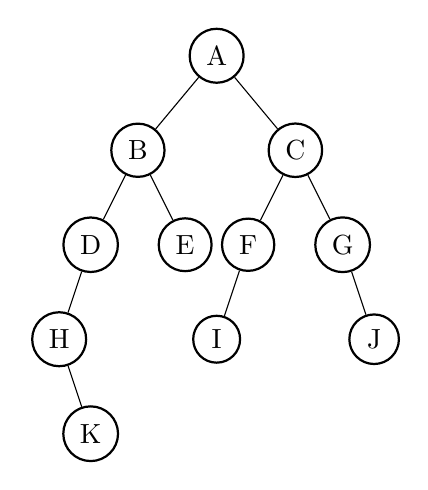
\begin{tikzpicture}[scale=0.8]

  %% \tikzstyle{every node}=[ball color=red!70,circle,text=white]

  %% \node [circle,draw] at (0,0) {A}; 

  \node[thick,circle,draw] at (0,0) {A}[sibling distance=4.8cm] 
  child { node[thick,circle,draw]{B}[sibling distance=2.4cm]
    child {node[thick,circle,draw]{D}[sibling distance=1.8cm]
      child {node[thick,circle,draw]{H}
        child[fill=none] {edge from parent[draw=none]}  
        child {node[thick,circle,draw]{K}}
      }
      child[fill=none] {edge from parent[draw=none]}  
    }
    child {node[thick,circle,draw]{E}}
  }
  child { node[thick,circle,draw]{C}[sibling distance=2.4cm]
    child {node[thick,circle,draw]{F}[sibling distance=1.8cm]
      child {node[thick,circle,draw]{I}}
      child[fill=none] {edge from parent[draw=none]}  
    }
    child {node[thick,circle,draw]{G}[sibling distance=1.8cm]
      child[fill=none] {edge from parent[draw=none]}  
      child {node[thick,circle,draw]{J}}
    }          			
  };
 
  
\end{tikzpicture}

\end{figure}

\end{frame}
%
\begin{frame}\ft{前序遍历}
假设visit函数实现打印功能,即
\lstinputlisting[
language=C,
]{Chapters/Ch04/Code/BiTree/Print.c}
\end{frame}
%
%
%
%
%
\begin{frame}\ft{中序遍历}
\textcolor{acolor5}{规则:}
若二叉树为空,则遍历结束;否则
\begin{itemize}
\item[(1)] 中序遍历左子树;
\item[(2)] 访问根结点;
\item[(3)] 中序遍历右子树。
\end{itemize}
\end{frame}
%
\begin{frame}[fragile]\ft{中序遍历}
\begin{figure}
\centering
\begin{tikzpicture}[scale=0.8]

  %% \tikzstyle{every node}=[ball color=red!70,circle,text=white]

  %% \node [circle,draw] at (0,0) {A}; 

  \node [circle,draw] at (0,0) (A) {A}[sibling distance=2.4cm] 
  child { node[circle,draw](B){B}[sibling distance=2.1cm]
    child {node[circle,draw](D){D}[sibling distance=1.8cm]
      child {node[circle,draw](G){G}}
      child {node[circle,draw](H){H}}
    }
    child[fill=none] {edge from parent[draw=none]}
  }
  child { node[circle,draw](C){C}[sibling distance=2.1cm]
    child {node[circle,draw](E){E}[sibling distance=1.8cm]
      child[fill=none] {edge from parent[draw=none]}  
      child {node[circle,draw](I){I}}
    }
    child {node[circle,draw](F){F}}          			
  };
  \pause 
  \draw[thick,blue,densely dashed,->,>=latex] (G)..controls +(100:1cm)  and +(190:1cm)..  node[] {\textcolor{acolor3} 1}(D);\pause     
  \draw[thick,blue,densely dashed,->,>=latex] (D)..controls +(260:1cm)  and +(170:1cm)..  node[] {\textcolor{acolor3} 2}(H);\pause     
  \draw[thick,blue,densely dashed,->,>=latex] (H)..controls +(100:1cm)  and +(260:1cm)..  node[] {\textcolor{acolor3} 3}(B);\pause     
  \draw[thick,blue,densely dashed,->,>=latex] (B)..controls +(100:1cm)  and +(200:1cm)..  node[] {\textcolor{acolor3} 4}(A);\pause     
  \draw[thick,blue,densely dashed,->,>=latex] (A)..controls +(260:1cm)  and +(100:1cm)..  node[] {\textcolor{acolor3} 5}(E);\pause
  \draw[thick,blue,densely dashed,->,>=latex] (E)..controls +(260:1cm)  and +(170:1cm)..  node[] {\textcolor{acolor3} 6}(I);\pause
  \draw[thick,blue,densely dashed,->,>=latex] (I)..controls +(100:1cm)  and +(260:1cm)..  node[] {\textcolor{acolor3} 7}(C);\pause
  \draw[thick,blue,densely dashed,->,>=latex] (C)..controls +(-30:1cm)  and +(100:1cm)..  node[] {\textcolor{acolor3} 8}(F);\pause

  \node [below=1] at (H) {
    \begin{lstlisting}
      `中序遍历结果:` G D H B A E I C F
    \end{lstlisting}
  };
  
\end{tikzpicture}

\end{figure}  
\end{frame}
%
%
%
\begin{frame}\ft{中序遍历}
\lstinputlisting[
language=C,
]{Chapters/Ch04/Code/BiTree/InOrderTraverse.c}

\end{frame}
%

\begin{frame}\ft{中序遍历}
\begin{zhu}
中序遍历,相对于前序遍历而言,只是把调用左孩子的递归函数提前了。
\end{zhu}
\end{frame}
%
%
%\begin{frame}\ft{\subsubsecname}
%\begin{itemize}
%\item[1] {\tt InOrderTraverse(tree, Print)}:访问根结点A;
%\item[]  {\tt InOrderTraverse(pnode->lchild, Print)}:访问结点B;
%\item[]  {\tt InOrderTraverse(pnode->lchild, Print)}:访问结点D;
%\item[]  {\tt InOrderTraverse(pnode->lchild, Print)}:访问结点H;
%\item[]  {\tt InOrderTraverse(pnode->lchild, Print)}:访问结点H的左孩子,不存在,返回至结点H,打印字母H。
%\end{itemize}
%\end{frame}
%
%
%\begin{frame}\ft{\subsubsecname}
%\begin{figure}
%\centering
%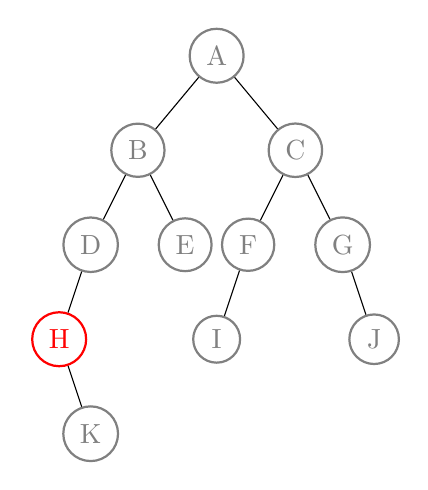
\begin{tikzpicture}[scale=0.8]

  %% \tikzstyle{every node}=[ball color=red!70,circle,text=white]

  %% \node [circle,draw] at (0,0) {A}; 

  \node[gray,thick,circle,draw] at (0,0) {A}[sibling distance=4.8cm] 
  child { node[gray,thick,circle,draw]{B}[sibling distance=2.4cm]
    child {node[gray,thick,circle,draw]{D}[sibling distance=1.8cm]
      child {node[red,thick,circle,draw]{H}
        child[fill=none] {edge from parent[draw=none]}  
        child {node[gray,thick,circle,draw]{K}}
      }
      child[fill=none] {edge from parent[draw=none]}  
    }
    child {node[gray,thick,circle,draw]{E}}
  }
  child { node[gray,thick,circle,draw]{C}[sibling distance=2.4cm]
    child {node[gray,thick,circle,draw]{F}[sibling distance=1.8cm]
      child {node[gray,thick,circle,draw]{I}}
      child[fill=none] {edge from parent[draw=none]}  
    }
    child {node[gray,thick,circle,draw]{G}[sibling distance=1.8cm]
      child[fill=none] {edge from parent[draw=none]}  
      child {node[gray,thick,circle,draw]{J}}
    }          			
  };
 
  
\end{tikzpicture}

%\end{figure} 
%\end{frame}
%
%
%\begin{frame}\ft{\subsubsecname}
%\begin{itemize}
%\item[2] 调用\tf InOrderTraverse(pnode->rchild, Print),访问结点H的右孩子K,因结点K无左孩子,故打印字母K。 
%\end{itemize}
%\begin{figure}
%\centering
%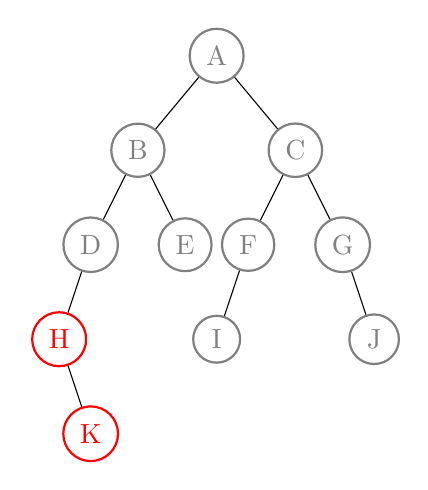
\begin{tikzpicture}[scale=0.8]

  %% \tikzstyle{every node}=[ball color=red!70,circle,text=white]

  %% \node [circle,draw] at (0,0) {A}; 

  \node[gray,thick,circle,draw] at (0,0) {A}[sibling distance=4.8cm] 
  child { node[gray,thick,circle,draw]{B}[sibling distance=2.4cm]
    child {node[gray,thick,circle,draw]{D}[sibling distance=1.8cm]
      child {node[red,thick,circle,draw]{H}
        child[fill=none] {edge from parent[draw=none]}  
        child {node[red,thick,circle,draw]{K}}
      }
      child[fill=none] {edge from parent[draw=none]}  
    }
    child {node[gray,thick,circle,draw]{E}}
  }
  child { node[gray,thick,circle,draw]{C}[sibling distance=2.4cm]
    child {node[gray,thick,circle,draw]{F}[sibling distance=1.8cm]
      child {node[gray,thick,circle,draw]{I}}
      child[fill=none] {edge from parent[draw=none]}  
    }
    child {node[gray,thick,circle,draw]{G}[sibling distance=1.8cm]
      child[fill=none] {edge from parent[draw=none]}  
      child {node[gray,thick,circle,draw]{J}}
    }          			
  };
 
  
\end{tikzpicture}

%\end{figure} 
%\end{frame}
%
%
%\begin{frame}\ft{\subsubsecname}
%\begin{itemize}
%\item[3] \tf 结点K没有右孩子,至此结点K访问完毕。返回至结点H,至此结点H也访问完毕。返回至D,打印字母D。
%\end{itemize}
%\begin{figure}
%\centering
%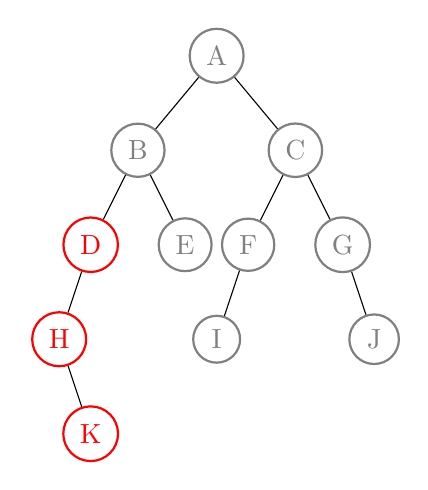
\begin{tikzpicture}[scale=0.8]

  %% \tikzstyle{every node}=[ball color=red!70,circle,text=white]

  %% \node [circle,draw] at (0,0) {A}; 

  \node[gray,thick,circle,draw] at (0,0) {A}[sibling distance=4.8cm] 
  child { node[gray,thick,circle,draw]{B}[sibling distance=2.4cm]
    child {node[red,thick,circle,draw]{D}[sibling distance=1.8cm]
      child {node[red,thick,circle,draw]{H}
        child[fill=none] {edge from parent[draw=none]}  
        child {node[red,thick,circle,draw]{K}}
      }
      child[fill=none] {edge from parent[draw=none]}  
    }
    child {node[gray,thick,circle,draw]{E}}
  }
  child { node[gray,thick,circle,draw]{C}[sibling distance=2.4cm]
    child {node[gray,thick,circle,draw]{F}[sibling distance=1.8cm]
      child {node[gray,thick,circle,draw]{I}}
      child[fill=none] {edge from parent[draw=none]}  
    }
    child {node[gray,thick,circle,draw]{G}[sibling distance=1.8cm]
      child[fill=none] {edge from parent[draw=none]}  
      child {node[gray,thick,circle,draw]{J}}
    }          			
  };
 
  
\end{tikzpicture}

%\end{figure} 
%\end{frame}
%
%
%\begin{frame}\ft{\subsubsecname}
%\begin{itemize}
%\item[4] \tf 结点D没有右孩子,至此结点D访问完毕。返回至结点B,打印字母B。
%\end{itemize}
%\begin{figure}
%\centering
%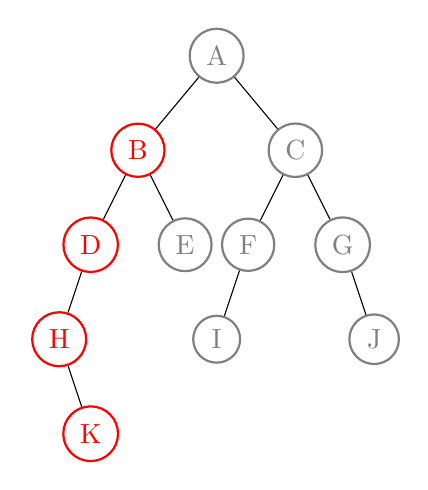
\begin{tikzpicture}[scale=0.8]

  %% \tikzstyle{every node}=[ball color=red!70,circle,text=white]

  %% \node [circle,draw] at (0,0) {A}; 

  \node[gray,thick,circle,draw] at (0,0) {A}[sibling distance=4.8cm] 
  child { node[red,thick,circle,draw]{B}[sibling distance=2.4cm]
    child {node[red,thick,circle,draw]{D}[sibling distance=1.8cm]
      child {node[red,thick,circle,draw]{H}
        child[fill=none] {edge from parent[draw=none]}  
        child {node[red,thick,circle,draw]{K}}
      }
      child[fill=none] {edge from parent[draw=none]}  
    }
    child {node[gray,thick,circle,draw]{E}}
  }
  child { node[gray,thick,circle,draw]{C}[sibling distance=2.4cm]
    child {node[gray,thick,circle,draw]{F}[sibling distance=1.8cm]
      child {node[gray,thick,circle,draw]{I}}
      child[fill=none] {edge from parent[draw=none]}  
    }
    child {node[gray,thick,circle,draw]{G}[sibling distance=1.8cm]
      child[fill=none] {edge from parent[draw=none]}  
      child {node[gray,thick,circle,draw]{J}}
    }          			
  };
 
  
\end{tikzpicture}

%\end{figure} 
%\end{frame}
%
%\begin{frame}\ft{\subsubsecname}
%\begin{itemize}
%\item[5] \tf 调用InOrderTraverse(pnode->rchild, Print),访问结点B的右孩子E,因结点E无左孩子,故打印字母E。
%\end{itemize}
%\begin{figure}
%\centering
%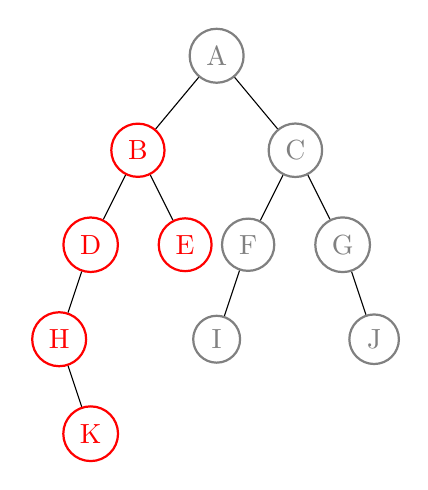
\begin{tikzpicture}[scale=0.8]

  %% \tikzstyle{every node}=[ball color=red!70,circle,text=white]

  %% \node [circle,draw] at (0,0) {A}; 

  \node[gray,thick,circle,draw] at (0,0) {A}[sibling distance=4.8cm] 
  child { node[red,thick,circle,draw]{B}[sibling distance=2.4cm]
    child {node[red,thick,circle,draw]{D}[sibling distance=1.8cm]
      child {node[red,thick,circle,draw]{H}
        child[fill=none] {edge from parent[draw=none]}  
        child {node[red,thick,circle,draw]{K}}
      }
      child[fill=none] {edge from parent[draw=none]}  
    }
    child {node[red,thick,circle,draw]{E}}
  }
  child { node[gray,thick,circle,draw]{C}[sibling distance=2.4cm]
    child {node[gray,thick,circle,draw]{F}[sibling distance=1.8cm]
      child {node[gray,thick,circle,draw]{I}}
      child[fill=none] {edge from parent[draw=none]}  
    }
    child {node[gray,thick,circle,draw]{G}[sibling distance=1.8cm]
      child[fill=none] {edge from parent[draw=none]}  
      child {node[gray,thick,circle,draw]{J}}
    }          			
  };
 
  
\end{tikzpicture}

%\end{figure} 
%\end{frame}
%
%\begin{frame}\ft{\subsubsecname}
%\begin{itemize}
%\item[6] \tf 结点E无右孩子,至此结点E访问完毕。返回至结点B,至此结点B也访问完毕。返回到结点A,打印字母A。
%\end{itemize}
%\begin{figure}
%\centering
%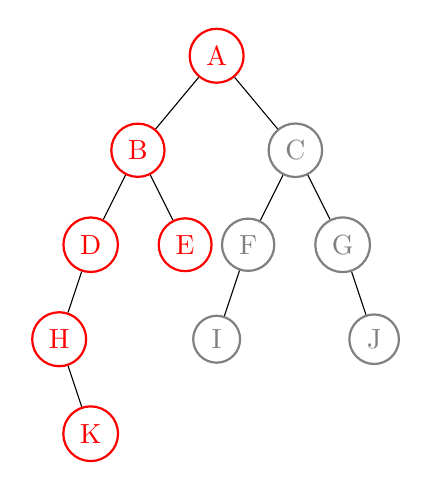
\begin{tikzpicture}[scale=0.8]

  %% \tikzstyle{every node}=[ball color=red!70,circle,text=white]

  %% \node [circle,draw] at (0,0) {A}; 

  \node[red,thick,circle,draw] at (0,0) {A}[sibling distance=4.8cm] 
  child { node[red,thick,circle,draw]{B}[sibling distance=2.4cm]
    child {node[red,thick,circle,draw]{D}[sibling distance=1.8cm]
      child {node[red,thick,circle,draw]{H}
        child[fill=none] {edge from parent[draw=none]}  
        child {node[red,thick,circle,draw]{K}}
      }
      child[fill=none] {edge from parent[draw=none]}  
    }
    child {node[red,thick,circle,draw]{E}}
  }
  child { node[gray,thick,circle,draw]{C}[sibling distance=2.4cm]
    child {node[gray,thick,circle,draw]{F}[sibling distance=1.8cm]
      child {node[gray,thick,circle,draw]{I}}
      child[fill=none] {edge from parent[draw=none]}  
    }
    child {node[gray,thick,circle,draw]{G}[sibling distance=1.8cm]
      child[fill=none] {edge from parent[draw=none]}  
      child {node[gray,thick,circle,draw]{J}}
    }          			
  };
 
  
\end{tikzpicture}

%\end{figure} 
%\end{frame}
%
%\begin{frame}\ft{\subsubsecname}
%\begin{itemize}
%\item[7] \tf 再调用InOrderTraverse(pnode->rchild, Print),访问结点A的右孩子C;
%\item[]      再调用InOrderTraverse(pnode->lchild, Print),访问结点C的左孩子F;
%\item[]      再调用InOrderTraverse(pnode->lchild, Print),访问结点F的左孩子I;
%\item[]      因结点I无左孩子,故打印字母I。
%\end{itemize}
%\end{frame}
%
%\begin{frame}\ft{\subsubsecname}
%\begin{figure}
%\centering
%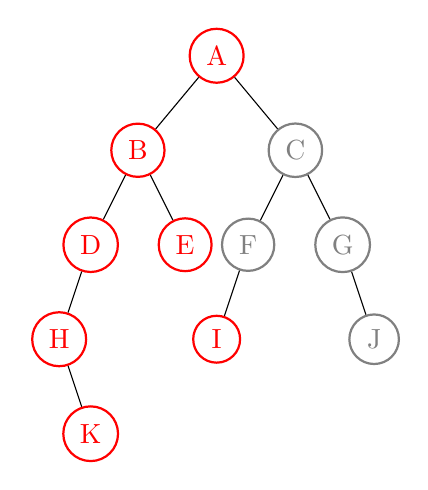
\begin{tikzpicture}[scale=0.8]

  %% \tikzstyle{every node}=[ball color=red!70,circle,text=white]

  %% \node [circle,draw] at (0,0) {A}; 

  \node[red,thick,circle,draw] at (0,0) {A}[sibling distance=4.8cm] 
  child { node[red,thick,circle,draw]{B}[sibling distance=2.4cm]
    child {node[red,thick,circle,draw]{D}[sibling distance=1.8cm]
      child {node[red,thick,circle,draw]{H}
        child[fill=none] {edge from parent[draw=none]}  
        child {node[red,thick,circle,draw]{K}}
      }
      child[fill=none] {edge from parent[draw=none]}  
    }
    child {node[red,thick,circle,draw]{E}}
  }
  child { node[gray,thick,circle,draw]{C}[sibling distance=2.4cm]
    child {node[gray,thick,circle,draw]{F}[sibling distance=1.8cm]
      child {node[red,thick,circle,draw]{I}}
      child[fill=none] {edge from parent[draw=none]}  
    }
    child {node[gray,thick,circle,draw]{G}[sibling distance=1.8cm]
      child[fill=none] {edge from parent[draw=none]}  
      child {node[gray,thick,circle,draw]{J}}
    }          			
  };
 
  
\end{tikzpicture}

%\end{figure}
%\end{frame}
%
%\begin{frame}\ft{\subsubsecname}
%\begin{itemize}
%\item[8] \tf之后分别打印F、C、G、J。
%\end{itemize}
%\end{frame}
%
%\subsubsection{后序遍历}
%
\begin{frame}\ft{后序遍历}
\textcolor{acolor5}{规则:}
若二叉树为空,则遍历结束;否则
\begin{itemize}
\item[(1)] 后序遍历左子树;
\item[(2)] 后序遍历右子树;
\item[(3)] 访问根结点。
\end{itemize}
\end{frame}
%
\begin{frame}[fragile]\ft{后序遍历}
\begin{figure}
\centering
\begin{tikzpicture}[scale=0.8]

  %% \tikzstyle{every node}=[ball color=red!70,circle,text=white]

  %% \node [circle,draw] at (0,0) {A}; 

  \node [circle,draw] at (0,0) (A) {A}[sibling distance=2.4cm] 
  child { node[circle,draw](B){B}[sibling distance=2.1cm]
    child {node[circle,draw](D){D}[sibling distance=1.8cm]
      child {node[circle,draw](G){G}}
      child {node[circle,draw](H){H}}
    }
    child[fill=none] {edge from parent[draw=none]}
  }
  child { node[circle,draw](C){C}[sibling distance=2.1cm]
    child {node[circle,draw](E){E}[sibling distance=1.8cm]
      child[fill=none] {edge from parent[draw=none]}  
      child {node[circle,draw](I){I}}
    }
    child {node[circle,draw](F){F}}          			
  };
  \pause 
  \draw[thick,blue,densely dashed,->,>=latex] (G)..controls +(0:1cm)    and +(180:1cm)..  node[] {\textcolor{acolor3} 1}(H);\pause     
  \draw[thick,blue,densely dashed,->,>=latex] (H)..controls +(80:1cm)   and +(-30:1cm)..  node[] {\textcolor{acolor3} 2}(D);\pause     
  \draw[thick,blue,densely dashed,->,>=latex] (D)..controls +(100:1cm)  and +(190:1cm)..  node[] {\textcolor{acolor3} 3}(B);\pause     
  \draw[thick,blue,densely dashed,->,>=latex] (B)..controls +(260:1cm)  and +(160:1.5cm)..node[] {\textcolor{acolor3} 4}(I);\pause     
  \draw[thick,blue,densely dashed,->,>=latex] (I)..controls +(100:1cm)  and +(-30:1cm)..  node[] {\textcolor{acolor3} 5}(E);\pause
  \draw[thick,blue,densely dashed,->,>=latex] (E)..controls +(0:1cm)    and +(180:1cm)..  node[] {\textcolor{acolor3} 6}(F);\pause
  \draw[thick,blue,densely dashed,->,>=latex] (F)..controls +(80:1cm)   and +(-30:1cm)..  node[] {\textcolor{acolor3} 7}(C);\pause
  \draw[thick,blue,densely dashed,->,>=latex] (C)..controls +(80:1cm)   and +(-30:1cm)..  node[] {\textcolor{acolor3} 8}(A);\pause

  \node [below=1] at (H) {
    \begin{lstlisting}
      `后序遍历结果:` G H D B I E F C A
    \end{lstlisting}
  };
  
\end{tikzpicture}

\end{figure} 
\end{frame}
%
%
%
\begin{frame}\ft{后序遍历}
\lstinputlisting[
language=C,
]{Chapters/Ch04/Code/BiTree/PostOrderTraverse.c}

\end{frame}
%
%\begin{frame}\ft{\subsubsecname}
%\begin{itemize}
%\item[1]   调用\tf InOrderTraverse(tree, Print),访问根结点A;
%\item[]  调用InOrderTraverse(pnode->lchild, Print),访问结点B;
%\item[]  调用InOrderTraverse(pnode->lchild, Print),访问结点D;
%\item[]  调用InOrderTraverse(pnode->lchild, Print),访问结点H;
%\item[]  调用InOrderTraverse(pnode->lchild, Print),访问结点H的左孩子,不存在,返回至结点H;
%\item[]  调用InOrderTraverse(pnode->rchild, Print),访问结点K;
%\item[]  调用InOrderTraverse(pnode->lchild, Print),访问结点K的左孩子,不存在,返回至结点K;
%\item[]  调用InOrderTraverse(pnode->lchild, Print),访问结点K的左孩子,不存在,返回至结点K,打印字母K,至此结点K访问完毕。
%\end{itemize}
%\end{frame}
%
%
%\begin{frame}\ft{\subsubsecname}
%\begin{figure}
%\centering
%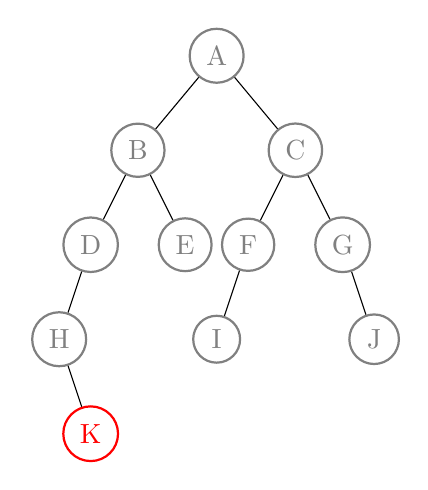
\begin{tikzpicture}[scale=0.8]

  %% \tikzstyle{every node}=[ball color=red!70,circle,text=white]

  %% \node [circle,draw] at (0,0) {A}; 

  \node[gray,thick,circle,draw] at (0,0) {A}[sibling distance=4.8cm] 
  child { node[gray,thick,circle,draw]{B}[sibling distance=2.4cm]
    child {node[gray,thick,circle,draw]{D}[sibling distance=1.8cm]
      child {node[gray,thick,circle,draw]{H}
        child[fill=none] {edge from parent[draw=none]}  
        child {node[red,thick,circle,draw]{K}}
      }
      child[fill=none] {edge from parent[draw=none]}  
    }
    child {node[gray,thick,circle,draw]{E}}
  }
  child { node[gray,thick,circle,draw]{C}[sibling distance=2.4cm]
    child {node[gray,thick,circle,draw]{F}[sibling distance=1.8cm]
      child {node[gray,thick,circle,draw]{I}}
      child[fill=none] {edge from parent[draw=none]}  
    }
    child {node[gray,thick,circle,draw]{G}[sibling distance=1.8cm]
      child[fill=none] {edge from parent[draw=none]}  
      child {node[gray,thick,circle,draw]{J}}
    }          			
  };
 
  
\end{tikzpicture}

%\end{figure} 
%\end{frame}
%
%
%\begin{frame}\ft{\subsubsecname}
%\begin{itemize}
%\item[2] \tf返回至结点H,打印字母H,至此结点H访问完毕。
%\end{itemize}
%\begin{figure}
%\centering
%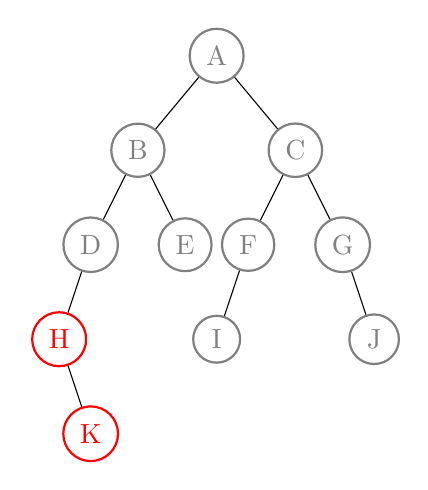
\begin{tikzpicture}[scale=0.8]

  %% \tikzstyle{every node}=[ball color=red!70,circle,text=white]

  %% \node [circle,draw] at (0,0) {A}; 

  \node[gray,thick,circle,draw] at (0,0) {A}[sibling distance=4.8cm] 
  child { node[gray,thick,circle,draw]{B}[sibling distance=2.4cm]
    child {node[gray,thick,circle,draw]{D}[sibling distance=1.8cm]
      child {node[red,thick,circle,draw]{H}
        child[fill=none] {edge from parent[draw=none]}  
        child {node[red,thick,circle,draw]{K}}
      }
      child[fill=none] {edge from parent[draw=none]}  
    }
    child {node[gray,thick,circle,draw]{E}}
  }
  child { node[gray,thick,circle,draw]{C}[sibling distance=2.4cm]
    child {node[gray,thick,circle,draw]{F}[sibling distance=1.8cm]
      child {node[gray,thick,circle,draw]{I}}
      child[fill=none] {edge from parent[draw=none]}  
    }
    child {node[gray,thick,circle,draw]{G}[sibling distance=1.8cm]
      child[fill=none] {edge from parent[draw=none]}  
      child {node[gray,thick,circle,draw]{J}}
    }          			
  };
 
  
\end{tikzpicture}

%\end{figure} 
%\end{frame}
%
%
%\begin{frame}\ft{\subsubsecname}
%\begin{itemize}
%\item[3] \tf返回至结点D,调用InOrderTraverse(pnode->rchild, Print)访问D的右孩子,因结点D无右孩子,返回至结点D,打印字母D,至此结点D访问完毕。
%\end{itemize}
%\begin{figure}
%\centering
%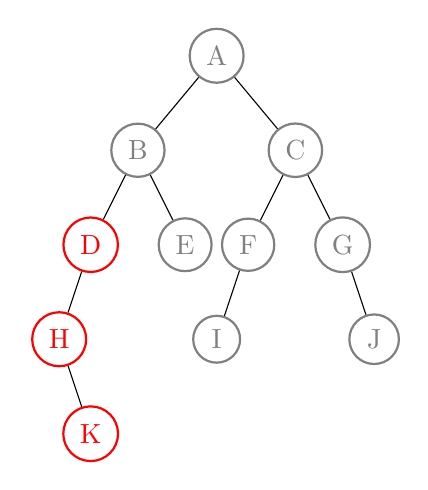
\begin{tikzpicture}[scale=0.8]

  %% \tikzstyle{every node}=[ball color=red!70,circle,text=white]

  %% \node [circle,draw] at (0,0) {A}; 

  \node[gray,thick,circle,draw] at (0,0) {A}[sibling distance=4.8cm] 
  child { node[gray,thick,circle,draw]{B}[sibling distance=2.4cm]
    child {node[red,thick,circle,draw]{D}[sibling distance=1.8cm]
      child {node[red,thick,circle,draw]{H}
        child[fill=none] {edge from parent[draw=none]}  
        child {node[red,thick,circle,draw]{K}}
      }
      child[fill=none] {edge from parent[draw=none]}  
    }
    child {node[gray,thick,circle,draw]{E}}
  }
  child { node[gray,thick,circle,draw]{C}[sibling distance=2.4cm]
    child {node[gray,thick,circle,draw]{F}[sibling distance=1.8cm]
      child {node[gray,thick,circle,draw]{I}}
      child[fill=none] {edge from parent[draw=none]}  
    }
    child {node[gray,thick,circle,draw]{G}[sibling distance=1.8cm]
      child[fill=none] {edge from parent[draw=none]}  
      child {node[gray,thick,circle,draw]{J}}
    }          			
  };
 
  
\end{tikzpicture}

%\end{figure} 
%\end{frame}
%
%
%\begin{frame}\ft{\subsubsecname}
%\begin{itemize}
%\item[4] \tf返回至结点B,调用InOrderTraverse(pnode->rchild, Print)访问B的右孩子E,因结点E无孩子,故打印字母E,至此结点E访问完毕。
%\end{itemize}
%\begin{figure}
%\centering
%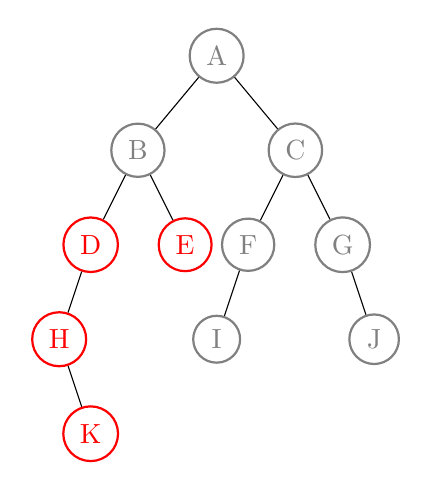
\begin{tikzpicture}[scale=0.8]

  %% \tikzstyle{every node}=[ball color=red!70,circle,text=white]

  %% \node [circle,draw] at (0,0) {A}; 

  \node[gray,thick,circle,draw] at (0,0) {A}[sibling distance=4.8cm] 
  child { node[gray,thick,circle,draw]{B}[sibling distance=2.4cm]
    child {node[red,thick,circle,draw]{D}[sibling distance=1.8cm]
      child {node[red,thick,circle,draw]{H}
        child[fill=none] {edge from parent[draw=none]}  
        child {node[red,thick,circle,draw]{K}}
      }
      child[fill=none] {edge from parent[draw=none]}  
    }
    child {node[red,thick,circle,draw]{E}}
  }
  child { node[gray,thick,circle,draw]{C}[sibling distance=2.4cm]
    child {node[gray,thick,circle,draw]{F}[sibling distance=1.8cm]
      child {node[gray,thick,circle,draw]{I}}
      child[fill=none] {edge from parent[draw=none]}  
    }
    child {node[gray,thick,circle,draw]{G}[sibling distance=1.8cm]
      child[fill=none] {edge from parent[draw=none]}  
      child {node[gray,thick,circle,draw]{J}}
    }          			
  };
 
  
\end{tikzpicture}

%\end{figure} 
%\end{frame}
%
%\begin{frame}\ft{\subsubsecname}
%\begin{itemize}
%\item[5] \tf返回至结点B,打印字母B,至此结点B访问完毕。
%\end{itemize}
%\begin{figure}
%\centering
%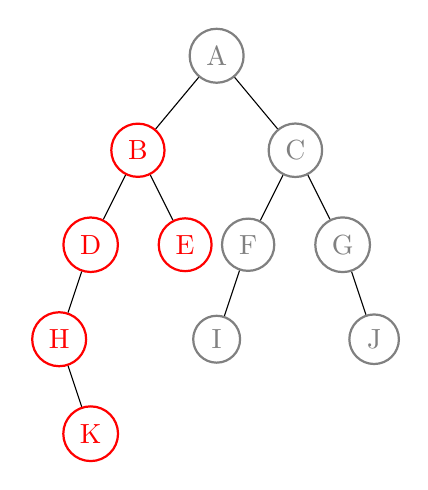
\begin{tikzpicture}[scale=0.8]

  %% \tikzstyle{every node}=[ball color=red!70,circle,text=white]

  %% \node [circle,draw] at (0,0) {A}; 

  \node[gray,thick,circle,draw] at (0,0) {A}[sibling distance=4.8cm] 
  child { node[red,thick,circle,draw]{B}[sibling distance=2.4cm]
    child {node[red,thick,circle,draw]{D}[sibling distance=1.8cm]
      child {node[red,thick,circle,draw]{H}
        child[fill=none] {edge from parent[draw=none]}  
        child {node[red,thick,circle,draw]{K}}
      }
      child[fill=none] {edge from parent[draw=none]}  
    }
    child {node[red,thick,circle,draw]{E}}
  }
  child { node[gray,thick,circle,draw]{C}[sibling distance=2.4cm]
    child {node[gray,thick,circle,draw]{F}[sibling distance=1.8cm]
      child {node[gray,thick,circle,draw]{I}}
      child[fill=none] {edge from parent[draw=none]}  
    }
    child {node[gray,thick,circle,draw]{G}[sibling distance=1.8cm]
      child[fill=none] {edge from parent[draw=none]}  
      child {node[gray,thick,circle,draw]{J}}
    }          			
  };
 
  
\end{tikzpicture}

%\end{figure} 
%\end{frame}
%
%\begin{frame}\ft{\subsubsecname}
%\begin{itemize}
%\item[6] \tf返回至结点A,调用InOrderTraverse(pnode->rchild, Print),访问A的右孩子C,
%\item[]   调用InOrderTraverse(pnode->lchild, Print),访问C的右孩子F,
%\item[]   调用InOrderTraverse(pnode->lchild, Print),访问F的右孩子I,因结点I无孩子,故打印字母I,至此结点I访问完毕。
%\end{itemize}
%\end{frame}
%
%\begin{frame}\ft{\subsubsecname}
%\begin{figure}
%\centering
%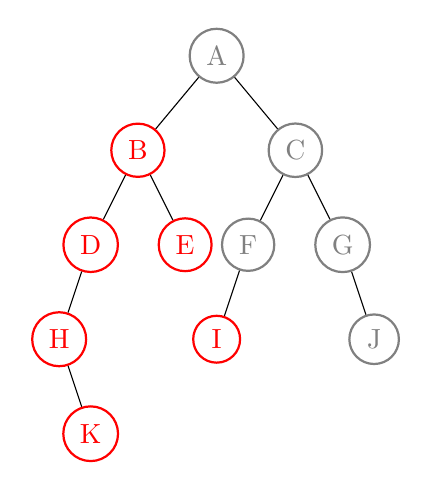
\begin{tikzpicture}[scale=0.8]

  %% \tikzstyle{every node}=[ball color=red!70,circle,text=white]

  %% \node [circle,draw] at (0,0) {A}; 

  \node[gray,thick,circle,draw] at (0,0) {A}[sibling distance=4.8cm] 
  child { node[red,thick,circle,draw]{B}[sibling distance=2.4cm]
    child {node[red,thick,circle,draw]{D}[sibling distance=1.8cm]
      child {node[red,thick,circle,draw]{H}
        child[fill=none] {edge from parent[draw=none]}  
        child {node[red,thick,circle,draw]{K}}
      }
      child[fill=none] {edge from parent[draw=none]}  
    }
    child {node[red,thick,circle,draw]{E}}
  }
  child { node[gray,thick,circle,draw]{C}[sibling distance=2.4cm]
    child {node[gray,thick,circle,draw]{F}[sibling distance=1.8cm]
      child {node[red,thick,circle,draw]{I}}
      child[fill=none] {edge from parent[draw=none]}  
    }
    child {node[gray,thick,circle,draw]{G}[sibling distance=1.8cm]
      child[fill=none] {edge from parent[draw=none]}  
      child {node[gray,thick,circle,draw]{J}}
    }          			
  };
 
  
\end{tikzpicture}

%\end{figure} 
%\end{frame}
%
%\begin{frame}\ft{\subsubsecname}
%\begin{itemize}
%\item[7] \tf返回至结点F,调用InOrderTraverse(pnode->rchild, Print),访问F的右孩子,因结点F无右孩子,故打印字母F,至此结点F访问完毕。
%\end{itemize}
%%% \end{frame}
%
%%% \begin{frame}\ft{\subsubsecname}
%\begin{figure}
%\centering
%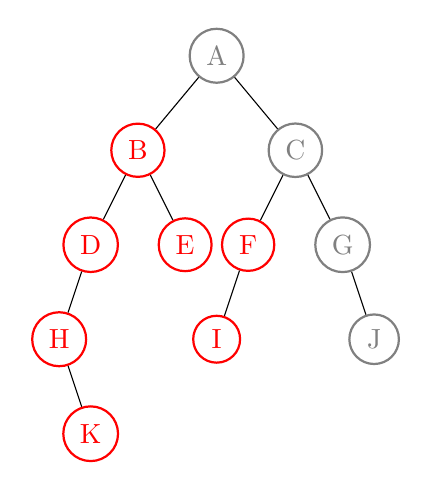
\begin{tikzpicture}[scale=0.8]

  %% \tikzstyle{every node}=[ball color=red!70,circle,text=white]

  %% \node [circle,draw] at (0,0) {A}; 

  \node[gray,thick,circle,draw] at (0,0) {A}[sibling distance=4.8cm] 
  child { node[red,thick,circle,draw]{B}[sibling distance=2.4cm]
    child {node[red,thick,circle,draw]{D}[sibling distance=1.8cm]
      child {node[red,thick,circle,draw]{H}
        child[fill=none] {edge from parent[draw=none]}  
        child {node[red,thick,circle,draw]{K}}
      }
      child[fill=none] {edge from parent[draw=none]}  
    }
    child {node[red,thick,circle,draw]{E}}
  }
  child { node[gray,thick,circle,draw]{C}[sibling distance=2.4cm]
    child {node[red,thick,circle,draw]{F}[sibling distance=1.8cm]
      child {node[red,thick,circle,draw]{I}}
      child[fill=none] {edge from parent[draw=none]}  
    }
    child {node[gray,thick,circle,draw]{G}[sibling distance=1.8cm]
      child[fill=none] {edge from parent[draw=none]}  
      child {node[gray,thick,circle,draw]{J}}
    }          			
  };
 
  
\end{tikzpicture}

%\end{figure}
%\end{frame}
%
%\begin{frame}\ft{\subsubsecname}
%\begin{itemize}
%\item[8] \tf之后分别打印J、G、C、A。
%\end{itemize}
%\end{frame}
%
%
%\begin{frame}[fragile]\ft{\subsecname}
%\begin{figure}
%\centering
%\begin{tikzpicture}[level distance=10mm]
  \tikzstyle{every node}=[circle,draw]
  \tikzstyle{level 1}=[sibling distance=2.5cm]
  \tikzstyle{level 2}=[sibling distance=1.5cm]
  \tikzstyle{level 3}=[sibling distance=1cm]

  \node[text width=0.3cm] at(2,0) {\tf -}
  child{node[text width=0.3cm]{\tf +}
    child{node[text width=0.3cm]{\tf a}}
    child{node[text width=0.3cm]{\tf *}
      child{node[text width=0.3cm]{\tf b}}
      child{node[text width=0.3cm]{\tf -}
        child{node[text width=0.3cm]{\tf c}}
        child{node[text width=0.3cm]{\tf d}}}}}
  child{node[text width=0.3cm]{\tf /}
    child{node[text width=0.3cm]{\tf e}}
    child{node[text width=0.3cm]{\tf f}}};

  \tikzstyle{every node}=[]
  \tikzstyle{information text}=[rounded corners,fill=blue!20!red!40,inner sep=1ex]
  \pause 
  \node [right,text width=5cm,style=information text
  ] at (5,0) {前序序列:
    \begin{lstlisting}[basicstyle=\tf\small]
 - + a * b - c d / e f
    \end{lstlisting}
  };

  \pause 
  \node [right,text width=5cm,style=information text
  ] at (5,-2) {中序序列:
    \begin{lstlisting}[basicstyle=\tf\small]
 a + b * c - d - e / f
    \end{lstlisting}
  };

  \pause 
  \node [right,text width=5cm,style=information text
  ] at (5,-4) {后序序列:
    \begin{lstlisting}[basicstyle=\tf\small]
 a b c d - * + e f / -
    \end{lstlisting}
  };

\end{tikzpicture}

%\caption{表达式{\tf (a+b*(c-d)-e/f)}的二叉树表示}
%\end{figure}
%\end{frame}
%
%\begin{frame}\ft{\subsecname}
%\begin{wenti}
%\tf已知一棵二叉树的前序遍历序列为A、B、C、D、E、F,中序遍历序列为C、B、A、E、D、F,请问这棵二叉树的后序遍历结果是多少?
%\end{wenti}
%%\pause
%
%\tf1. 由前序遍历序列A、B、C、D、E、F可知,A为根结点。由中序遍历序列C、B、A、E、D、F知,C、B为A的左子树结点,E、D、F为A的右子树结点。
%\begin{figure}
%\centering
%\begin{tikzpicture}[scale=0.8]

  \tikzstyle{every node}=[thick,draw]

  %% \node [circle,draw] at (0,0) {A}; 

  \node[circle] at (0,0) {A}[sibling distance=3cm] 
  child { node[ellipse,text width=1.2cm]{B、C}}
  child { node[ellipse,text width=1.2cm]{D、E、F}};
\end{tikzpicture}

%\end{figure}
%\end{frame}
%
%\begin{frame}\ft{\subsecname}
%%% \begin{wenti}
%%%   \tf已知一棵二叉树的前序遍历序列为A、B、C、D、E、F,中序遍历序列为C、B、A、E、D、F,请问这棵二叉树的后序遍历结果是多少?
%%% \end{wenti}
%%% %\pause
%
%\tf2. 先看前序中的B、C,是先打印B后打印C,故B是A的左孩子,而C是B的孩子,但是左是右不能确定。再看中序的C、B,C在B之前打印,故C是B的左孩子。
%\begin{figure}
%\centering
%\begin{tikzpicture}[scale=0.8]

  \tikzstyle{every node}=[thick,draw]

  %% \node [circle,draw] at (0,0) {A}; 

  \node[circle] at (0,0) {A}[sibling distance=3cm] 
  child { node[circle]{B}
    child{ node[circle] {C}}
    child[fill=none] {edge from parent[draw=none]}  
  }
  child { node[ellipse,text width=1.2cm]{D、E、F}};
\end{tikzpicture}

%\end{figure}
%\end{frame}
%
%
%\begin{frame}\ft{\subsecname}
%%% \begin{wenti}
%%%   \tf已知一棵二叉树的前序遍历序列为A、B、C、D、E、F,中序遍历序列为C、B、A、E、D、F,请问这棵二叉树的后序遍历结果是多少?
%%% \end{wenti}
%%% %\pause
%
%\tf3. 先看前序中的D、E、F,意味着D是A的右孩子,而E、F是D的后代。再看中序序列中的E、D、F,可以确定E是D的左孩子,F是D的右孩子。于是得到了最终的二叉树,其后续遍历结果为\red{C、B、E、F、D、A。}
%\begin{figure}
%\centering
%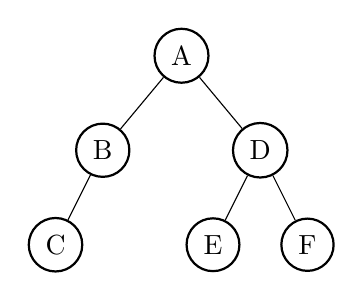
\begin{tikzpicture}[scale=0.8]

  \tikzstyle{every node}=[thick,draw]

  %% \node [circle,draw] at (0,0) {A}; 

  \node[circle] at (0,0) {A}[sibling distance=3cm] 
  child { node[circle]{B}
    child{ node[circle] {C}}
    child[fill=none] {edge from parent[draw=none]}  
  }
  child { node[circle]{D}
    child{ node[circle] {E}}
    child{ node[circle] {F}}
  };
\end{tikzpicture}

%\end{figure}
%\end{frame}
%
%
%
\begin{frame}\ft{\secname}
\begin{wenti}
已知一棵二叉树的中序遍历序列为D、G、B、H、E、I、A、C、J、F,后序遍历序列为G、D、H、I、E、B、J、F、C、A,请问这棵二叉树的前序遍历结果是多少?
\end{wenti}
\pause
\textcolor{acolor3}{解:}1. 由后序遍历序列可知,A为根结点。由中序遍历序列知,D、G、B、H、E、I为A的左子树结点,C、J、F为A的右子树结点。
\begin{figure}
\centering
\begin{tikzpicture}[scale=0.8]

  \tikzstyle{every node}=[thick,draw]

  %% \node [circle,draw] at (0,0) {A}; 

  \node[circle] at (0,0) {A}[sibling distance=6.8cm] 
  child { node[ellipse]{D、G、B、H、E、I}}
  child { node[ellipse]{C、J、F}};
\end{tikzpicture}

\end{figure}
\end{frame}
%
\begin{frame}\ft{\secname}
2. 看A的左子树,由中序序列D、G、B、H、E、I和后序序列G、D、H、I、E、B,知B是该子树的根结点,且D、G为B的左子树结点,H、E、I为B的右子树结点。
\begin{figure}
\centering
\begin{tikzpicture}[scale=0.8]

  \tikzstyle{every node}=[thick,draw]

  \node[circle] at (0,0) {A}[sibling distance=4cm] 
  child { node[circle]{B}[sibling distance=3cm] 
    child{ node[ellipse] {D、G}}
    child{ node[ellipse] {H、E、I}}
  }
  child { node[ellipse,text width=1.2cm]{C、J、F}};
\end{tikzpicture}

\end{figure}
\end{frame}
%
%
\begin{frame}\ft{\secname}  
3. 看B的左子树,由中序序列D、G和后序序列G、D知,D为该子树的根结点,且G为D的右孩子。
\begin{figure}
\centering
\begin{tikzpicture}[scale=0.8]

  \tikzstyle{every node}=[thick,draw]

  \node[circle] at (0,0) {A}[sibling distance=4cm] 
  child { node[circle]{B}[sibling distance=3cm] 
    child{ node[ellipse] {D}[sibling distance=2cm]
      child[fill=none] {edge from parent[draw=none]}  
      child{ node[ellipse] {G}}
    }
    child{ node[ellipse] {H、E、I}}
  }
  child { node[ellipse,text width=1.2cm]{C、J、F}};
\end{tikzpicture}

\end{figure}
\end{frame}

\begin{frame}\ft{\secname}  
4. 看B的右子树,由中序序列H、E、I和后序序列H、I、E知,E为该子树的根结点,且H为E的左孩子,I为E的右孩子。
\begin{figure}
\centering
\begin{tikzpicture}[scale=0.8]

  \tikzstyle{every node}=[thick,draw]

  \node[circle] at (0,0) {A}[sibling distance=4cm] 
  child { node[circle]{B}[sibling distance=3cm] 
    child{ node[circle] {D}[sibling distance=2cm]
      child[fill=none] {edge from parent[draw=none]}  
      child{ node[circle] {G}}
    }
    child{ node[circle] {E}[sibling distance=2cm]
      child{ node[circle] {H}}
      child{ node[circle] {I}}
    }
  }
  child { node[ellipse]{C、J、F}};
\end{tikzpicture}

\end{figure}
\end{frame}

\begin{frame}\ft{\secname}  
5. 看A的右子树,由中序序列C、J、F和后序序列J、F、C知,C为该子树的根结点,J、F为C的右子树结点。
\begin{figure}
\centering
\begin{tikzpicture}[scale=0.8]

  \tikzstyle{every node}=[thick,draw]

  \node[circle] at (0,0) {A}[sibling distance=4cm] 
  child { node[circle]{B}[sibling distance=3cm] 
    child{ node[circle] {D}[sibling distance=2cm]
      child[fill=none] {edge from parent[draw=none]}  
      child{ node[circle] {G}}
    }
    child{ node[circle] {E}[sibling distance=2cm]
      child{ node[circle] {H}}
      child{ node[circle] {I}}
    }
  }
  child { node[ellipse]{C}
    child[fill=none] {edge from parent[draw=none]}  
    child{ node[ellipse] {F、J}}
  };
\end{tikzpicture}

\end{figure}
\end{frame}

\begin{frame}\ft{\secname}  
6. 看C的右子树,由中序序列J、F和后序序列J、F知,F为该子树的根结点,且J为F的左孩子。
\begin{figure}
\centering
\begin{tikzpicture}[scale=0.8]

  \tikzstyle{every node}=[thick,draw]

  \node[circle] at (0,0) {A}[sibling distance=4cm] 
  child { node[circle]{B}[sibling distance=3cm] 
    child{ node[circle] {D}[sibling distance=2cm]
      child[fill=none] {edge from parent[draw=none]}  
      child{ node[circle] {G}}
    }
    child{ node[circle] {E}[sibling distance=2cm]
      child{ node[circle] {H}}
      child{ node[circle] {I}}
    }
  }
  child { node[ellipse]{C}[sibling distance=3cm] 
    child[fill=none] {edge from parent[draw=none]}  
    child{ node[ellipse] {F}[sibling distance=2cm]
      child{ node[ellipse] {J}}
      child[fill=none] {edge from parent[draw=none]}  
    }
  };
\end{tikzpicture}

\end{figure}
\end{frame}
%
\begin{frame}\ft{\secname}  
\begin{wenti}
已知一棵二叉树的前序序列为A、B、C,后序序列为C、B、A,请问这棵二叉树的中序遍历结果是多少?
\end{wenti}
\pause

\textcolor{acolor3}{解:}由前序序列和后序序列可以确定根结点为A,但接下来无法确定哪个结点是左子树,哪个是右子树。%\pause
这棵树有以下四种可能:
\begin{figure}
\centering
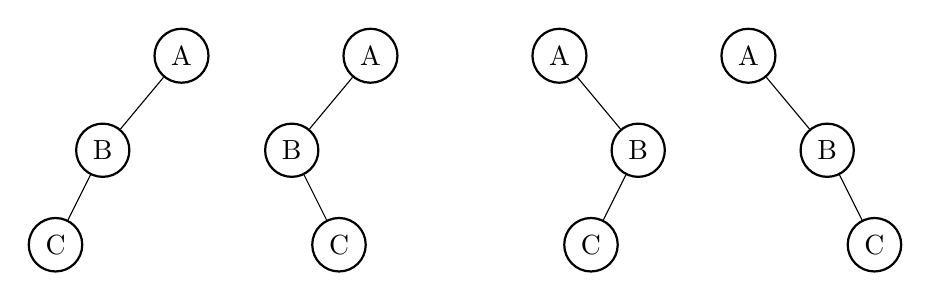
\begin{tikzpicture}[scale=0.8]

  \tikzstyle{every node}=[thick,draw]
  \node[circle] at (0,0) {A}
  child { node[circle]{B}
    child { node[circle]{C}}
    child[fill=none] {edge from parent[draw=none]}  
  }
  child[fill=none] {edge from parent[draw=none]};

  \node[circle] at (3,0) {A}
  child { node[circle]{B}
    child[fill=none] {edge from parent[draw=none]}  
    child { node[circle]{C}}
  }
  child[fill=none] {edge from parent[draw=none]};


  \node[circle] at (6,0) {A}
  child[fill=none] {edge from parent[draw=none]}
  child { node[circle]{B}
    child { node[circle]{C}}
    child[fill=none] {edge from parent[draw=none]}  
  };

  \node[circle] at (9,0) {A}
  child[fill=none] {edge from parent[draw=none]}
  child { node[circle]{B}
    child[fill=none] {edge from parent[draw=none]}
    child { node[circle]{C}}
  };

\end{tikzpicture}

\end{figure}

\end{frame}


\begin{frame}\ft{\subsecname}
\textcolor{acolor5}{二叉树遍历的性质:}
\begin{itemize}
\item 已知前序遍历序列和中序遍历序列,可以唯一确定一棵二叉树;\\[0.1in]
\item 已知后序遍历序列和中序遍历序列,可以唯一确定一棵二叉树;\\[0.1in]
\item 已知前序遍历序列和后序遍历序列,不能确定一棵二叉树。
\end{itemize}
\end{frame}
%
%\subsubsection{层次遍历}
\begin{frame}\ft{层次遍历}
\textcolor{acolor5}{规则:}
若二叉树为空,则遍历结束;否则从树的第一层,也就是根节点开始访问,从上而下逐层遍历,在同一层中,按从左到右的顺序对结点逐个访问。
\end{frame}
%
\begin{frame}[fragile]\ft{层次遍历}
\begin{figure}
\centering
\begin{tikzpicture}[scale=0.8]

  %% \tikzstyle{every node}=[ball color=red!70,circle,text=white]

  %% \node [circle,draw] at (0,0) {A}; 

  \node [circle,draw] at (0,0) (A) {A}[sibling distance=2.4cm] 
  child { node[circle,draw](B){B}[sibling distance=2.1cm]
    child {node[circle,draw](D){D}[sibling distance=1.8cm]
      child {node[circle,draw](G){G}}
      child {node[circle,draw](H){H}}
    }
    child[fill=none] {edge from parent[draw=none]}
  }
  child { node[circle,draw](C){C}[sibling distance=2.1cm]
    child {node[circle,draw](E){E}[sibling distance=1.8cm]
      child[fill=none] {edge from parent[draw=none]}  
      child {node[circle,draw](I){I}}
    }
    child {node[circle,draw](F){F}}          			
  };
  \pause 
  \draw[thick,blue,densely dashed,->,>=latex] (A)..controls +(190:1cm) and +(110:1cm)..  node[] {\textcolor{acolor3} 1}(B);\pause     
  \draw[thick,blue,densely dashed,->,>=latex] (B)..controls +(0:1cm)   and +(180:1cm)..  node[] {\textcolor{acolor3} 2}(C);\pause     
  \draw[thick,blue,densely dashed,->,>=latex] (C)..controls +(190:1cm) and +(40:1cm)..   node[] {\textcolor{acolor3} 3}(D);\pause     
  \draw[thick,blue,densely dashed,->,>=latex] (D)..controls +(0:1cm)   and +(180:1cm)..  node[] {\textcolor{acolor3} 4}(E);\pause     
  \draw[thick,blue,densely dashed,->,>=latex] (E)..controls +(0:1cm)   and +(180:1cm)..  node[] {\textcolor{acolor3} 5}(F);\pause
  \draw[thick,blue,densely dashed,->,>=latex] (F)..controls +(190:1cm) and +(30:1cm)..   node[] {\textcolor{acolor3} 6}(G);\pause
  \draw[thick,blue,densely dashed,->,>=latex] (G)..controls +(0:1cm)  and +(180:1cm)..   node[] {\textcolor{acolor3} 7}(H);\pause
  \draw[thick,blue,densely dashed,->,>=latex] (H)..controls +(0:1cm)  and +(180:1cm)..   node[] {\textcolor{acolor3} 8}(I);\pause

  \node [below=1] at (H) {
    \begin{lstlisting}
      `前序遍历结果:` A B D G H C E I F
    \end{lstlisting}
  };
  
\end{tikzpicture}

\end{figure} 
\end{frame}
%
\begin{frame}[fragile,allowframebreaks]\ft{层次遍历}

\lstinputlisting[
language=C,
]{Chapters/Ch04/Code/BiTree/LevelOrderTraverse.c}

\end{frame}
%


